\documentclass[12,english]{article}
\usepackage[letterpaper, portrait, margin=1in]{geometry}
\usepackage{amsmath}
\usepackage[T1]{fontenc}
\usepackage{babel}
\usepackage{textcomp}
\usepackage{titlesec}
\setcounter{secnumdepth}{4}
\usepackage{hyperref}
\usepackage{xcolor}
\usepackage{booktabs}
\usepackage{placeins}
\usepackage{graphicx}
\usepackage{tabularx}
\usepackage{amsmath}
\usepackage[T1]{fontenc}
\usepackage{babel}
\usepackage{textcomp}
\usepackage{titlesec}
\setcounter{secnumdepth}{4}
\usepackage{hyperref}
\usepackage{color}
\hypersetup{
    bookmarks=true,     
      colorlinks=true,     
    linkcolor=black,      
    citecolor=green,     
    filecolor=magenta,    
    urlcolor=cyan        
}

\titleformat{\paragraph}
{\normalfont\normalsize\bfseries}{\theparagraph}{1em}{}
\titlespacing*{\paragraph}
{0pt}{3.25ex plus 1ex minus .2ex}{1.5ex plus .2ex}

\title{Test Report for Group 15 - Flight Shooting Game}
\author{Yijun Chen\\
\texttt{ (cheny161)}
\and
Tianxing Li\\
\texttt{(lit20)}
\and
Zefeng Wang\\
\texttt{(wangz217)}
}

\date{}


\begin{document}
\maketitle
\newpage
\tableofcontents
\newpage

\section{Revision History}					

%PUT LATEST CHANGES FIRST e.g. revision 2, 1, 0.

\begin{table}[!htbp]

	\begin{tabular}[r]{|l|l|l|}

		\hline		
		\textbf{Revision} & \textbf{Date} & \textbf{Change}\\ 
		\hline
		\color{red}3 & \color{red}12/05/18 & \color{red}Final Rev 1 \\
		\hline
		0 & 11/05/18 & Draft Complete \\ \hline


	\end{tabular}
		\caption{Revision history for Test Report document}
		\label{Table}
\end{table}
	
\section{List of Tables and Figures}
	Table 1 - Revision History\\
	Table 2...21 - Test Cases\\
	Table 22 - Trace to Requirements\\
	Table 22 - Trace to Modules \\

\section{Functional Qualities Evaluation}

	Description of Tests: The purpose of these tests is to ensure that the user is able to use the software according to the given requirements. These tests will include direction control testing, collision testing, ultimate testing, start, restart and quit testing.\\ \\
	
	Test Name: FS-PC-2 \\
	
	Results: The user is able to move around the flight by pressing "WASD" or direction keys. \\ \\
	
	Test Name: FS-R-3 \\
	
	Results: The user is able to collide with enemy flights and enemy bullets to lose health points. \\ \\
	
	Test Name: FS-PC-17 \\
	
	Results: The user is able to press "U" on keyboard to use ultimate when the ultimate condition is ready. After the use of ultimate, all enemies already on the will lose 3500 health points.\\ \\
	
	Test Name: FS-MC-1 \\
	
	Results: The user is able to press "SPACE" to enter the game at the start page. \\ \\
	
	Test Name: FS-MC-2 \\
	
	Results: The user is able to press "R" to restart the game at the end page. All game data will be reset and the game goes to the start page.\\ \\
	
	Test Name: FS-MC-3 \\
	
	Results: The user is able to press "Q" to quit the game at the end page. The game window will be closed right after pressing the key.\\ \\
	

\section{Non-functional Qualities Evaluation} 	\subsection{GUI Testing}
Description of Test: Usability of the Graphical User Interface (GUI) was tested by a small test group of ten McMaster students who are not in Software Engineering but are instead from different backgrounds (i.e.  Social Sciences) to better reflect the technological experience of the potential users for this program. Participants were monitored to observe the time it took them to perform the requested task. After the participants were finished with all tasks, each participant gives feedback to the developers verbally.

	\subsubsection{Look and feel}
	Test Name: NF-L-1 )\\
	Results: All participants were able to successfully complete the task and tell the difficulty level of the enemies. However, the difficulty level between head boss and chramp boss are too close according to the feedback. 
	\subsubsection{usability}
	
	Test Name: NF-U-1\\
	Results: All the participants were able to successfully complete the task. According to the feedback, the game control keys are pretty common and popular from the existing games.

	\subsubsection{Performance}
	Test Name: NF-P-1 \\
	Results: According to the feedback, no latency or slow response occurred during game play.
	
	\subsubsection{Operational and Environmental}

	Test Name: NF-O-1 \\
	Results: No content that would violate  culture, religion or politics was found.\\
	
\section{Automated Testing}
For this part, \emph{unittest} library from Python is used. For each module in the system, a test code is written and conducted. Functional methods in such module are tested.\\\\
Description of tests for each module:\\\\
Given a module M and its set of functional methods S where $m_n$ $\in$ S.\\\\
Create a unit test class T with a set of n test cases TC where $c_n$ $\in$ TC.\\\\
Each test case refers to a module method.
$$c_n \Longleftrightarrow m_n$$
Each test case with a module method get a test result:
$$Conduct(c_n, m_n)\Rightarrow bool$$
True refers to pass and False refers to fail.\\\\
Here is the list of the functions for unit testing:\\\\
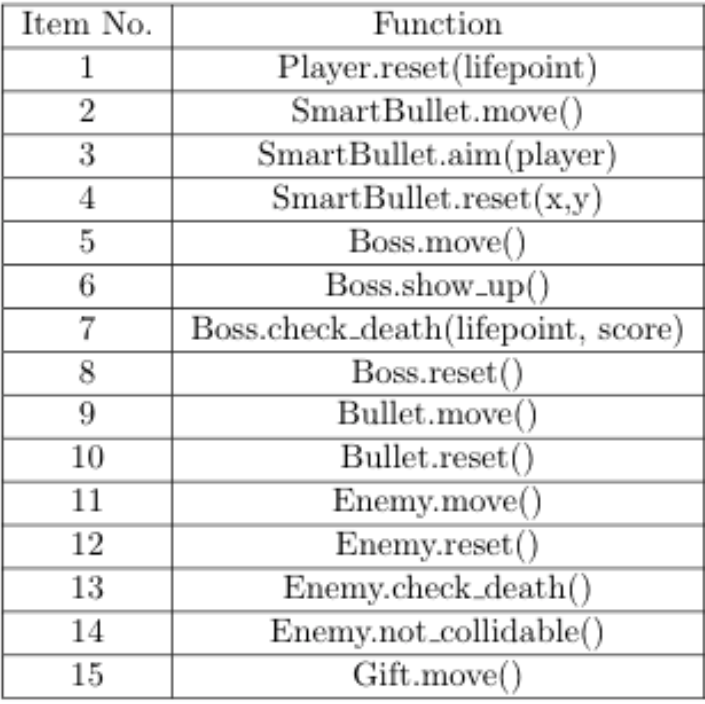
\includegraphics[scale=0.6]{ut.png}\\\\
Result: The end results of the testing were positive and all 15 test cases passed.
\section{System Test}
	\subsection{User Control Testing}
	
		\begin{table}[!htbp]
			
			\begin{tabular}[r]{|l|l|}
				
				\hline
				%\label
				
				\textbf{Test Name} & FS-PC-1 \\ 
				\hline
				\textbf{Initial State} & Game is running and player plane stays still at the bottom of the window. \\ 
				\hline
				\textbf{Input} & “W” or “UP” button. \\ 
				\hline 
				\textbf{Expected Output} & The player plane moves up for certain distance in range of 1/5 of the window vertically.  \\ 
				\hline
				
			\end{tabular}
			\caption{Test for FS-PC-1}
			\label{Table}
		\end{table}
		
		\begin{table}[!htbp]
			
			\begin{tabularx}{\textwidth}{|l|X|}
				
				\hline
				%\label
				
				\textbf{Test Name} & FS-PC-2
				\\ 
				\hline
				\textbf{Initial State} & A graph of player plane stays still at the bottom of the window. \\ 
				\hline
				\textbf{Input} & “W” or “UP” button. (Hold)  \\ 
				\hline 
				\textbf{Expected Output} & The player plane keeps moving up until it reach the top of the screen \\ 
				\hline
				
			\end{tabularx}
			\caption{Test for FS-PC-2}
			\label{Table}
		\end{table}

		\begin{table}[!htbp]
			
			\begin{tabularx}{\textwidth}{|l|X|}
				
				\hline
				%\label
				
				\textbf{Test Name} & FS-PC-3..4
				\\ 
				\hline
				\textbf{Initial State} & A graph of player plane stays still at the bottom of the window. \\ 
				\hline
				\textbf{Input} & “S” or “Down” button. (Hold)  \\ 
				\hline 
				\textbf{Expected Output} & The player plane keeps moving up until it reach the bottom of the screen \\ 
				\hline
				
			\end{tabularx}
			\caption{Test for FS-PC-3..4}
			\label{Table}
		\end{table}
				\begin{table}[!htbp]
			
			\begin{tabularx}{\textwidth}{|l|X|}
				
				\hline
				%\label
				
				\textbf{Test Name} & FS-PC-5..6
				\\ 
				\hline
				\textbf{Initial State} & A graph of player plane stays still at the bottom of the window. \\ 
				\hline
				\textbf{Input} & “A” or “Left” button. (Hold)  \\ 
				\hline 
				\textbf{Expected Output} & The player plane keeps moving up until it reach the left border of the screen \\ 
				\hline
				
			\end{tabularx}
			\caption{Test for FS-PC-5..6}
			\label{Table}
		\end{table}
				\begin{table}[!htbp]
			
			\begin{tabularx}{\textwidth}{|l|X|}
				
				\hline
				%\label
				
				\textbf{Test Name} & FS-PC-7..8
				\\ 
				\hline
				\textbf{Initial State} & A graph of player plane stays still at the bottom of the window. \\ 
				\hline
				\textbf{Input} & “D” or “Right” button. (Hold)  \\ 
				\hline 
				\textbf{Expected Output} & The player plane keeps moving up until it reach the right border of the screen \\ 
				\hline
				
			\end{tabularx}
			\caption{Test for FS-PC-7..8}
			\label{Table}
		\end{table}
				\begin{table}[!htbp]
			
			\begin{tabularx}{\textwidth}{|l|X|}
				
				\hline
				%\label
				
				\textbf{Test Name} & FS-PC-9..10
				\\ 
				\hline
				\textbf{Initial State} & A graph of player plane stays still at the bottom of the window. \\ 
				\hline
				\textbf{Input} & “W and A” or “UP and LEFT” button. (Hold)  \\ 
				\hline 
				\textbf{Expected Output} & The player plane keeps moving up until it reach the border of the screen \\ 
				\hline
				
			\end{tabularx}
			\caption{Test for FS-PC-9..10}
			\label{Table}
		\end{table}
				\begin{table}[!htbp]
			
			\begin{tabularx}{\textwidth}{|l|X|}
				
				\hline
				%\label
				
				\textbf{Test Name} & FS-PC-11..12
				\\ 
				\hline
				\textbf{Initial State} & A graph of player plane stays still at the bottom of the window. \\ 
				\hline
				\textbf{Input} & “W and D” or “UP and RIGHT” button. (Hold)  \\ 
				\hline 
				\textbf{Expected Output} & The player plane keeps moving up until it reach the border of the screen \\ 
				\hline
				
			\end{tabularx}
			\caption{Test for FS-PC-11..12}
			\label{Table}
		\end{table}
				\begin{table}[!htbp]
			
			\begin{tabularx}{\textwidth}{|l|X|}
				
				\hline
				%\label
				
				\textbf{Test Name} & FS-PC-13..14
				\\ 
				\hline
				\textbf{Initial State} & A graph of player plane stays still at the bottom of the window. \\ 
				\hline
				\textbf{Input} & “S and A” or “DOWN and LEFT” button. (Hold)  \\ 
				\hline 
				\textbf{Expected Output} & The player plane keeps moving up until it reach the border of the screen \\ 
				\hline
				
			\end{tabularx}
			\caption{Test for FS-PC-13..14}
			\label{Table}
		\end{table}
				\begin{table}[!htbp]
			
			\begin{tabularx}{\textwidth}{|l|X|}
				
				\hline
				%\label
				
				\textbf{Test Name} & FS-PC-15..16
				\\ 
				\hline
				\textbf{Initial State} & A graph of player plane stays still at the bottom of the window. \\ 
				\hline
				\textbf{Input} & “S and D” or “DOWN and RIGHT” button. (Hold)  \\ 
				\hline 
				\textbf{Expected Output} & The player plane keeps moving up until it reach the border of the screen \\ 
				\hline
				
			\end{tabularx}
			\caption{Test for FS-PC-15..16}
			\label{Table}
		\end{table}
				\begin{table}[!htbp]
			
			\begin{tabularx}{\textwidth}{|l|X|}
				
				\hline
				%\label
				
				\textbf{Test Name} & FS-PC-17
				\\ 
				\hline
				\textbf{Initial State} & Game running and play is alive with full “energy” and certain enemy planes on the field.\\ 
				\hline
				\textbf{Input} & “U" button. (Press once)  \\ 
				\hline 
				\textbf{Expected Output} & All the enemy planes should be destroyed instantly.
How test will be performed: When “energy” is full, player press “U” once and all enemy planes not including the boss alive are destroyed instantly. If any stay alive, there is an error. \\ 
				\hline
				
			\end{tabularx}
			\caption{Test for FS-PC-17}
			\label{Table}
		\end{table}
				\begin{table}[!htbp]
			
			\begin{tabularx}{\textwidth}{|l|X|}
				
				\hline
				%\label
				
				\textbf{Test Name} & FS-MC-1
				\\ 
				\hline
				\textbf{Initial State} & The game is on the start page. \\ 
				\hline
				\textbf{Input} & “SPACE” key. (Press once)  \\ 
				\hline 
				\textbf{Expected Output} & The game enters the game page and the game starts.
How test will be performed: When it is on the start page, press “SPACE” once, the game starts immediately. If there is any other behaviours, there is an error. \\ 
				\hline
				
			\end{tabularx}
			\caption{Test for FS-MC-1}
			\label{Table}
		\end{table}
				\begin{table}[!htbp]
			
			\begin{tabularx}{\textwidth}{|l|X|}
				
				\hline
				%\label
				
				\textbf{Test Name} & FS-MC-2
				\\ 
				\hline
				\textbf{Initial State} & The game is on the death page. \\ 
				\hline
				\textbf{Input} &“Q” key. (Press once) \\ 
				\hline 
				\textbf{Expected Output} & The game quits immediately.
How test will be performed: When the game is on death page, press “Q” once to quit the game. The windows should be closed. \\ 
				\hline
				
			\end{tabularx}
			\caption{Test for FS-MC-2}
			\label{Table}
		\end{table}
				\begin{table}[!htbp]
			
			\begin{tabularx}{\textwidth}{|l|X|}
				
				\hline
				%\label
				
				\textbf{Test Name} & FS-MC-3
				\\ 
				\hline
				\textbf{Initial State} & The game is at the death page. \\ 
				\hline
				\textbf{Input} & “R” key. (Press once)  \\ 
				\hline 
				\textbf{Expected Output} & The game restarts immediately.
How test will be performed: When the game is on death page, press “R” once to restart the game. A new game should start. \\ 
				\hline
				
			\end{tabularx}
			\caption{Test for FS-MC-3}
			\label{Table}
		\end{table}
				\begin{table}[!htbp]
			
			\begin{tabularx}{\textwidth}{|l|X|}
				
				\hline
				%\label
				
				\textbf{Test Name} & FS-PC-2
				\\ 
				\hline
				\textbf{Initial State} & A graph of player plane stays still at the bottom of the window. \\ 
				\hline
				\textbf{Input} & “W” or “UP” button. (Hold)  \\ 
				\hline 
				\textbf{Expected Output} & The player plane keeps moving up until it reach the top of the screen \\ 
				\hline
				
			\end{tabularx}
			\caption{Test for FS-PC-2}
			\label{Table}
		\end{table}
		
				\begin{table}[!htbp]
			
			\begin{tabularx}{\textwidth}{|l|X|}
				
				\hline
				%\label
				
				\textbf{Test Name} & FS-PC-2
				\\ 
				\hline
				\textbf{Initial State} & A graph of player plane stays still at the bottom of the window. \\ 
				\hline
				\textbf{Input} & “W” or “UP” button. (Hold)  \\ 
				\hline 
				\textbf{Expected Output} & The player plane keeps moving up until it reach the top of the screen \\ 
				\hline
				
			\end{tabularx}
			\caption{Test for FS-PC-2}
			\label{Table}
		\end{table}
	
		
\newpage
\subsection{System Control Testing}
\begin{table}[!htbp]
\begin{tabular}{|c|c|}
\hline
\textbf{Test Name} & FSR1\\
\hline
\textbf{Initial State} &The game on the start page.\\
\hline
\textbf{Input} &Play one round\\
\hline
\textbf{Expected Output}&Modification on high mark\\
\hline
\end{tabular}
\caption{Test for FSR1}
\label{Table}
\end{table}

\begin{table}[!htbp]
\begin{tabular}{|c|c|}
\hline
\textbf{Test Name} &FSR2\\
\hline
\textbf{Initial State} &The game is running and player is alive\\
\hline
\textbf{Input} &None\\
\hline
\textbf{Expected Output}&The player plane is shooting automatically\\
\hline
\end{tabular}
\caption{Test for FSR2}
\label{Table}
\end{table}

\begin{table}[!htbp]
\begin{tabular}{|c|c|}
\hline
\textbf{Test Name} & FSR3\\
\hline
\textbf{Initial State} &The game is running and player is alive\\
\hline
\textbf{Input} &Some operations to make the player's plane collide other enemy objects\\
\hline
\textbf{Expected Output}&Loss of life point\\
\hline
\end{tabular}
\caption{Test for FSR3}
\label{Table}
\end{table}

\begin{table}[!htbp]
\begin{tabular}{|c|c|}
\hline
\textbf{Test Name} & FSR4\\
\hline
\textbf{Initial State} &The game is running and player is alive\\
\hline
\textbf{Input} &Some operations making the player plane collide with gift object\\
\hline
\textbf{Expected Output}&add life point with ``+" sign gift\\
& power up fire with ``R" sigh gift\\
\hline
\end{tabular}
\caption{Test for FSR4}
\label{Table}
\end{table}

\section{Changes Due to Testing}				


	\subsection{GUI Testing}
	After conducting look and feel on GUI, the following changed are applied to differentiate the difficulty level between head boss and chramp boss:\\
	\\
	The image of chramp boss has been modified to look more aggressive\\
	\\
	
	\subsection{Unit testing}
	After conducting Unit test, no modification need to be applied. 

\section{Trace to Requirements}				

	
		\begin{table}[!htbp]
			\begin{tabular}{ll}
				\toprule
				Test & Requirements \\
				\midrule
				\multicolumn{2}{c}{Functional Requirements Testing} \\
				\midrule
				FS-PC-1-16 & FR1,FR2,FR3,FR4,FR5,FR6,FR7,FR8,FR9,FR10 \\
				FS-PC-(2...16) & FR7 \\
				FS-PC-17 & FR8 \\
				FS-MC-(1...3) & FR4 \\
	
				\midrule
				\multicolumn{2}{c}{Non-functional Requirements Testing} \\
				\midrule
				NF-L-1 & NF1,NF2,NF3,\\
				NF-U-1 & NF4, NF5, NF6,NF7,NF8,NF9, \\
				NF-P-1 & NF10, NF11, NF13,NF14,NF15, \\
				NP-O-1 & NF20, NF24, NF25,NF26,NF27 \\
				\midrule
				\multicolumn{2}{c}{Automated Testing} \\
				\midrule
				UF-1 & FR9\\
				UF-2 & FR9\\
				UF-3 & FR10\\
				UF-4 & FR10\\
				UF-5 & FR8,FR10 \\
				UF-6 & FR10\\
				UF-7 & FR10\\
				UF-8 & FR8\\
				UF-9 & FR5\\
				UF-10 & FR5\\
				UF-11 & FR8\\
				UF-12 & FR12\\
				UF-13 & FR9\\
				UF-14 & FR6\\
				\bottomrule
			\end{tabular}
			\caption{Trace Between Tests and Requirements}
			\makeatletter
			\def\rulecolor#1#{\CT@arc{#1}}
			\def\CT@arc#1#2{%
				\ifdim\baselineskip=\z@\noalign\fi
				{\gdef\CT@arc@{\color#1{#2}}}}
			\let\CT@arc@\relax
			\rulecolor{black!50}
			\makeatother
			\label{Table}
		\end{table}
		
		\FloatBarrier
	
	\newpage

\section{Trace to Modules}		% EVERYONE - reference MG

\begin{table}[!htbp]
	\begin{tabular}{ll}
		\toprule
		Test & Modules \\
		\midrule
		\multicolumn{2}{c}{Functional Requirements Testing} \\
		\midrule
		FS-PC-1-16 & M1...M7 \\
		FS-PC-(2...16) & M1...M7 \\
		FS-PC-17 & M1...M7 \\
		FS-MC-(1...3) & M1...M7 \\
		\midrule
		\multicolumn{2}{c}{Non-functional Requirements Testing} \\
		\midrule
		NF-L-1 & M1...M7,\\
		NF-U-1 & M1...M7\\
		NF-P-1 & M5 \\	
		NF-O-1 & M1...M7\\
		\midrule
		\multicolumn{2}{c}{Automated Testing} \\
		\midrule
		UF-1 & M5\\
		UF-2 & M3\\
		UF-3 & M3\\
		UF-4 & M3\\
		UF-5 & M1\\
		UF-6 & M1\\
		UF-7 & M1\\
		UF-8 & M1\\
		UF-9 & M2\\
		UF-10 & M2\\
		UF-11 & M4\\
		UF-12 & M4\\
		UF-13 & M4\\
		UF-14 & M6\\
		\bottomrule
	\end{tabular}
	\caption{Trace Between Tests and Modules}
	\makeatletter
	\def\rulecolor#1#{\CT@arc{#1}}
	\def\CT@arc#1#2{%
		\ifdim\baselineskip=\z@\noalign\fi
		{\gdef\CT@arc@{\color#1{#2}}}}
	\let\CT@arc@\relax
	\rulecolor{black!50}
	\makeatother
	\label{Table}
\end{table}

\FloatBarrier
	
	
\section{Code Coverage Metrics}				

	The Flight Shooting Game group has managed to produce roughly 90 percent code coverage through our tests. This number is based off the fact that all of the modules have been covered in testing along with the output. Please refer to the trace to modules section. There it is clearly shown that we have covered every module multiple times, once again confirming the 90 percent coverage rate.






\end{document}
